\newpage % Rozdziały zaczynamy od nowej strony.
\cleardoublepage % Zaczynamy od nieparzystej strony
\pagestyle{headings}

\section{Wybór sprzętu}

Dlaczego Sztuczne Sieci Neuronowe odpala się na GPU?
Dlaczego nie CPU i GPU tylko FPGA?
Typically, neural networks are designed, trained, and executed on a conventional processor, often with GPU acceleration. But for embedded devices which may need to process data at multiple-MHz sample rates, the computational requirements can be overwhelming for an embedded processor where no GPU is available, creating a tempting opportunity for FPGA acceleration. (https://github.com/Xilinx/RFNoC-HLS-NeuralNet)
Co z ASIC, dlaczego rzadko się je stosuje, jak wygląda proces tworzenia?
Dlaczego PC ma swoje ograniczenia? Jakie możliwości mają nowe algorytmy uruchamiane na PC?
Jaką przewagę dają układy FPGA, skąd się to bierze? porównanie zużycia mocy itp..\\

Trzeba tu tylko uważać, żeby nie powielać tekstu z rozdziału cel i zakres pracy.


\begin{table}[h] \centering
  \caption{Porównanie cen płytek z układami Zynq firmy Xilinx}
  \centering
  \begin{tabular} {c|c|c} \hline \label{tab:ceny}
      Nazwa płytki & Układ SoC & Cena \\ \hline
      Z-turn Board MYS-7Z010-C-S & XC7Z010-1CLG400C & 99\$\tablefootnote{http://www.myirtech.com/list.asp?id=502} \\ 
      Z-turn Board MYS-7Z020-C-S & XC7Z020-1CLG400C  & 119\$\footnotemark[1] \\
      Zybo Z7-10 Development Board & XC7Z010-1CLG400C & 199\$\tablefootnote{https://store.digilentinc.com/zybo-z7-zynq-7000-arm-fpga-soc-development-board/} \\
      Zybo Z7-20 Development Board & XC7Z020-1CLG400C & 299\$\footnotemark[2] \\
      ZedBoard Zynq-7000 & XC7Z020-CLG484-1 & 449\$\tablefootnote{https://store.digilentinc.com/zedboard-zynq-7000-arm-fpga-soc-development-board/} \\
  \end{tabular}
\end{table}


\subsection{Z-turn Board}

Z-turn Board (Rys. \ref{zturn_board} jest komputerem jednopłytkowym (ang. SBC – \emph{Single Board Computer}),
opartym o układ SoC Xilinx Zynq-7020 (XC7Z020-1CLG400C), zawierający dwurdzeniowy 
procesor ARM Cortex-A9 i układ FPGA Artix 7. 

\begin{figure}[h]
  \centering
  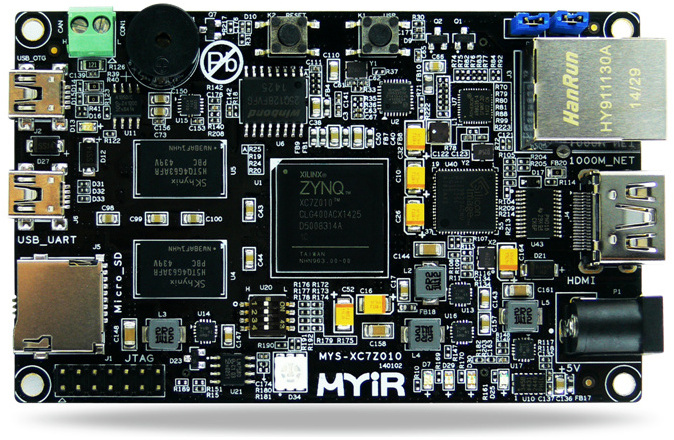
\includegraphics[width=0.5\textwidth]{img/zturn_board.jpg}
  \caption{Płytka Z-turn-Board 7020}
  \label{zturn_board}
\end{figure}

Biorąc pod uwagę parametry, płytka 
charakteryzuje się wysokim stodunkiem ceny do jakości, podstawowa wersja kosztuje 
99\$. Dla porównania płytka Zybo Z7-20 kosztuje 199\$. Zestawienie cen płytek 
zawierających układ Zynq XC7Z010 oraz XC7Z020 znajduje się w Tabeli \ref{tab:ceny}. 

\subsubsection{Interfejsy komunikacji}

Płytka Z-turn posiada interfejsy UART oraz Ethernet, które zostały wykorzystane do 
komunikacji komputera PC z systemem przy użyciu portu szeregowego  
i protokołu SSH (ang. \emph{Secure Shell}). Istnieje również możliwość podłączenia 
wyświetlacza bezpośrednio do płytki przy użyciu portu HDMI. Dodatkowo producent 
oferuje płytkę rozszerzeniową Z-turn IO-Cape (Rys. \ref{iocape}), która zawiera 
porty do podłączenia kamery przez protokół DVP (ang. \emph{Digital Video Port}) 
oraz wyświetlacza LCD. 

\begin{figure}[h]
  \centering
  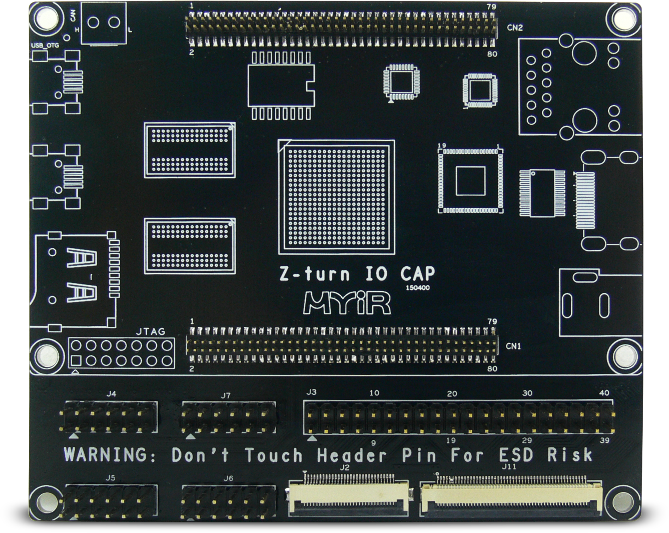
\includegraphics[width=0.5\textwidth]{img/iocape.png}
  \caption{Płytka rozszerzeniowa Z-turn IO Cape}
  \label{iocape}
\end{figure}

\subsection{Kamera}

\subsection{Xilinx Platform Cable}

\subsection{Opcje bootowania systemu}

